\documentclass[11pt]{article}

\usepackage{amsthm,amsmath,amsfonts,amssymb}
\usepackage[authoryear]{natbib}
\usepackage[colorlinks,citecolor=blue,urlcolor=blue,linkcolor=blue]{hyperref}
\usepackage{graphicx}
\usepackage{listings}
\usepackage{lstbayes}
\usepackage{xcolor}
\usepackage{booktabs}
\usepackage{pdflscape}
\usepackage{afterpage}
\usepackage[margin=1in,letterpaper]{geometry}

\lstset{language=Stan,
           basicstyle=\ttfamily\scriptsize,
           keywordstyle=\color{blue}\ttfamily\scriptsize,
           stringstyle=\color{red}\ttfamily\scriptsize,
           commentstyle=\color{gray}\ttfamily\scriptsize,
          breaklines=true
          }

\renewcommand{\thefigure}{S\arabic{figure}}
\renewcommand{\thetable}{S\arabic{table}}
\renewcommand{\thesection}{S\arabic{section}}

\begin{document}

\title{Supplementary Information for\\``Bayesian inference of the climbing grade scale''\\\large Manuscript ID DGJQAS.2026.0040}
\author{[Removed for blind review]}
\date{}
\maketitle

\section{Stan model}
\label{si:stan}

The Stan model used for all 20 analyses is shown in Listing~\ref{si:stan-listing}. The model corresponds to the dynamic Bradley-Terry formulation in Section~3 of the main text: each ascent's success indicator is a Bernoulli with logit link in $m \cdot (C_j(t) - x_i)$, where $x_i$ is the (observed) route grade, $C_j(t)$ is the (latent) grade of the climber at the time of the ascent, and $m$ is the slope parameter common to all climbers in the analysis. The prior on $m$ is a weakly informative log-normal placing its central 95\% mass on the interval $m \in [0.19, 1.97]$. The prior on each climber-month grade is a normal centred on the previous month's grade with standard deviation $w = 0.5$ (the discretised Wiener process), reverting to a wide normal centred on a per-dataset grade prior $\mu_0$ for months outside the climber's data window.

\begin{lstlisting}[language=Stan,caption={Stan model.},label=si:stan-listing]
data {
  int<lower=1> C;            // number of climbers
  int<lower=1> N;            // number of ascents
  int<lower=1> P;            // number of pages (months)
  int<lower=1> minPage[C];   // min page for each climber
  int<lower=1> maxPage[C];   // max page for each climber
  int<lower=0,upper=1> y[N]; // ascent success/failure
  int<lower=1> page[N];      // the time block (page) of each ascent
  int<lower=1> c[N];         // the climber of each ascent
  vector[N] x;               // route grade of each ascent
  int meanGradePrior;        // the mean of the grade prior
}
parameters {
  real climberGrade[C, P];   // latent climber grade per month
  real<lower=0.0> m;         // slope of increase in difficulty per grade increment
}
model {
  m ~ lognormal(-0.5, 0.6);  // prior on slope
  for (j in 1:C) {
    for (i in 1:minPage[j]) {
      climberGrade[j, i] ~ normal(meanGradePrior, 5);
    }
    for (i in (minPage[j]+1):maxPage[j]) {
      climberGrade[j, i] ~ normal(climberGrade[j, i-1], 0.5);
    }
    for (i in (maxPage[j]+1):P) {
      climberGrade[j, i] ~ normal(meanGradePrior, 5);
    }
  }
  for (i in 1:N) {
    y[i] ~ bernoulli_logit(m * (climberGrade[c[i], page[i]] - x[i]));
  }
}
\end{lstlisting}

All analyses were run with 4 parallel chains, 4{,}000 iterations per chain, of which the first 2{,}000 were discarded as warmup, leaving 8{,}000 total post-warmup draws. We monitored convergence with rank-normalised split-$\hat{R}$ and bulk/tail effective sample sizes following \citet{vehtari2021rank}.


\section{Cross-dataset summary}
\label{si:cross-dataset}

Table~\ref{si:datasets} reports, for each of the 20 analyses, the number of climbers retained ($n$), the number of logged ascents ($N$), the posterior median and 95\% equal-tail credible interval for $d = e^m$, and the inclusion threshold.

The selection pipeline retains climbers passing the per-attempt minimum thresholds (set to $30$ attempts and $1$ explicit failure for all 20 analyses). If more than $100$ climbers pass these thresholds, only the top-$100$ by total ascent count are kept; otherwise all eligible climbers are retained. In Table~\ref{si:datasets}, $n$ is shown in bold ($\mathbf{100}$) for the analyses where this top-$100$ cap was reached, and in normal weight where all eligible climbers were used.

The distinction matters for the threshold sensitivity reported in Section~5.1 of the main text: where the cap was reached, raising the attempt threshold to $\geq\!50$ or $\geq\!100$ has no effect because the top-$100$ most-active climbers all log many hundreds of attempts and are unaffected by any of these thresholds; where the cap was not reached, the threshold is the active selection rule. Of the 20 analyses, $10$ reached the cap (all 8 Australian analyses and both German UIAA-graded analyses) and $10$ did not (all 8 New Zealand analyses and both German French-graded analyses). The slope estimates are mutually consistent across this stratification: where the cap was not reached, the slope estimates are broadly similar to their cap-reached counterparts at the same country/style, suggesting that the cap acts as a computational ceiling rather than a substantive analytical choice.

\afterpage{%
    \clearpage
    \thispagestyle{empty}
    \begin{landscape}
    \begin{table}[ht]
    \centering
    \footnotesize
    \begin{tabular}{llllrrrrrr}
      \toprule
      {\bf Country} & {\bf Style} & {\bf Grade scale} & {\bf Game} & {$n$} & {$N$} & {$d=e^m$} & {2.5\%} & {97.5\%} & {\bf Min.\ attempts} \\
      \midrule
      Australia   & Boulder    & V-grade & attempt & $\mathbf{100}$ & $25{,}805$ & $2.96$ & $2.85$ & $3.07$ & $\geq 30$ \\
      Australia   & Boulder    & V-grade & session & $\mathbf{100}$ & $25{,}344$ & $3.03$ & $2.91$ & $3.15$ & $\geq 30$ \\
      Australia   & Sport      & Ewbank  & attempt & $\mathbf{100}$ & $52{,}947$ & $2.24$ & $2.21$ & $2.28$ & $\geq 30$ \\
      Australia   & Sport      & Ewbank  & session & $\mathbf{100}$ & $48{,}679$ & $2.33$ & $2.29$ & $2.37$ & $\geq 30$ \\
      Australia   & Sport+Trad & Ewbank  & attempt & $\mathbf{100}$ & $61{,}931$ & $2.13$ & $2.10$ & $2.16$ & $\geq 30$ \\
      Australia   & Sport+Trad & Ewbank  & session & $\mathbf{100}$ & $57{,}512$ & $2.18$ & $2.15$ & $2.21$ & $\geq 30$ \\
      Australia   & Trad       & Ewbank  & attempt & $\mathbf{100}$ & $14{,}929$ & $2.02$ & $1.96$ & $2.09$ & $\geq 30$ \\
      Australia   & Trad       & Ewbank  & session & $\mathbf{100}$ & $14{,}479$ & $2.01$ & $1.95$ & $2.08$ & $\geq 30$ \\
      \midrule
      New Zealand & Boulder    & V-grade & attempt & $15$  & $1{,}049$  & $3.35$ & $2.71$ & $4.27$ & $\geq 30$ \\
      New Zealand & Boulder    & V-grade & session & $15$  & $1{,}027$  & $3.35$ & $2.68$ & $4.32$ & $\geq 30$ \\
      New Zealand & Sport      & Ewbank  & attempt & $89$  & $10{,}027$ & $2.19$ & $2.11$ & $2.27$ & $\geq 30$ \\
      New Zealand & Sport      & Ewbank  & session & $89$  & $9{,}679$  & $2.22$ & $2.13$ & $2.31$ & $\geq 30$ \\
      New Zealand & Sport+Trad & Ewbank  & attempt & $98$  & $11{,}389$ & $2.15$ & $2.08$ & $2.22$ & $\geq 30$ \\
      New Zealand & Sport+Trad & Ewbank  & session & $98$  & $11{,}024$ & $2.17$ & $2.09$ & $2.26$ & $\geq 30$ \\
      New Zealand & Trad       & Ewbank  & attempt & $8$   & $524$      & $1.80$ & $1.57$ & $2.11$ & $\geq 30$ \\
      New Zealand & Trad       & Ewbank  & session & $8$   & $517$      & $1.77$ & $1.55$ & $2.07$ & $\geq 30$ \\
      \midrule
      Germany     & Sport      & French  & attempt & $8$   & $521$      & $2.08$ & $1.79$ & $2.46$ & $\geq 30$ \\
      Germany     & Sport      & French  & session & $8$   & $483$      & $2.09$ & $1.79$ & $2.49$ & $\geq 30$ \\
      Germany     & Sport      & UIAA    & attempt & $\mathbf{100}$ & $19{,}497$ & $2.12$ & $2.06$ & $2.18$ & $\geq 30$ \\
      Germany     & Sport      & UIAA    & session & $\mathbf{100}$ & $18{,}435$ & $2.14$ & $2.08$ & $2.21$ & $\geq 30$ \\
      \bottomrule
    \end{tabular}
    \caption{Summary of all 20 Bayesian analyses. $n$ is the number of climbers retained; $N$ is the number of logged ascents on which inference is performed (after per-session aggregation where applicable); $d = e^m$ is the posterior median multiplicative factor in difficulty per grade increment, with the 2.5\% and 97.5\% quantiles of the posterior shown as endpoints of a 95\% equal-tail credible interval. The minimum-attempts column lists the per-climber inclusion threshold (set to $30$ in all 20 analyses; the minimum-explicit-failures threshold is $1$ throughout). $n$ is shown in bold ($\mathbf{100}$) where the analysis was capped at the top-$100$ most-active climbers because more than $100$ climbers passed the inclusion thresholds; in the remaining analyses (where $n$ is shown in normal weight), all eligible climbers were used. The slope estimates are mutually consistent across this stratification, suggesting the cap acts as a computational ceiling rather than a substantive analytical choice.}
    \label{si:datasets}
    \end{table}
    \end{landscape}
    \clearpage
}


\section{Per-climber log-odds-ratio regression}
\label{si:regression}

The dynamic Bradley-Terry model in the main text assumes that the log-odds-ratio of failure is a linear function of the difference between the climber's grade and the route's grade, with slope $m$ common to all climbers. As a simple check on this assumption, and as the source of the per-climber log-linear slope estimates quoted in Section~5.1 of the main text ($0.65$ for the Australia-Sport per-session data set; $0.52$ for the New Zealand-Sport per-session data set), we fit an ordinary log-linear regression of $\log(\#\text{failures}/\#\text{successes})$ against route grade for each climber individually, treating each climber's grade as constant across the analysis window.

Figure~\ref{si:regression-aus} shows the resulting per-climber regression lines for the Australia-Sport per-session data set, and Figure~\ref{si:regression-nz} shows the same for New Zealand-Sport per-session. The slopes are broadly consistent across climbers despite the intercepts varying by approximately $10$ grades, supporting the choice of a shared slope parameter. The mean per-climber slopes ($0.65$ for AUS, $0.52$ for NZ) are below the joint Bayesian posterior estimates ($0.85$ for AUS, $0.80$ for NZ); we do not interpret this gap as a contradiction because the two estimators differ in important ways: the per-climber regression discards within-climber temporal structure (treating $C_j$ as constant), pools across the entire $5$-year window irrespective of activity, and uses ordinary least squares on data that is not exchangeable; the joint Bayesian model, by contrast, accounts for time-varying ability via the dynamic Bradley-Terry structure and pools information across climbers. The figures should therefore be read as a qualitative model-fit check rather than as a competing estimator.

\begin{figure}[htbp]
\centering
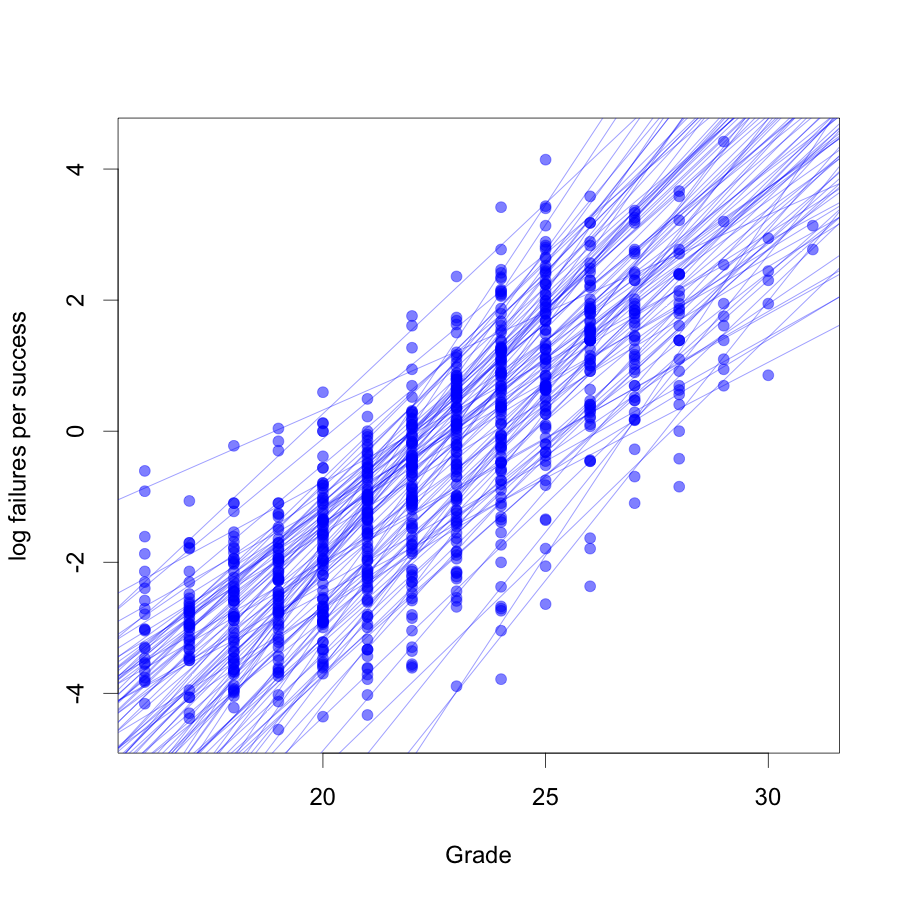
\includegraphics[width=0.85\textwidth]{figures/aus/ascents-from-2016-08-01-to-2021-08-01-minAscents30-minFails1-Sport-AU-session-regression.png}
\caption{Per-climber log-odds-ratio of failure versus route grade for the Australia-Sport per-session data set. Each point plots $\log(\#\text{failures}/\#\text{successes})$ at one grade for one climber; one regression line is fitted per climber. The slopes are visibly consistent across climbers, while the intercepts span a range of approximately $10$ grades.}
\label{si:regression-aus}
\end{figure}

\begin{figure}[htbp]
\centering

\includegraphics[width=0.85\textwidth]{figures/nz/ascents-from-2016-08-01-to-2021-08-01-minAscents30-minFails1-Sport-AU-session-regression.png}
\caption{Per-climber log-odds-ratio of failure versus route grade for the New Zealand-Sport per-session data set. Conventions as in Figure~\ref{si:regression-aus}.}
\label{si:regression-nz}
\end{figure}


\section{Convergence diagnostics for the main analysis}
\label{si:diagnostics}

Table~\ref{si:diag-aus-sport} reports convergence diagnostics for the main Australia-Sport per-session analysis (row 4 of Table~\ref{si:datasets}). Diagnostics are reported following \citet{vehtari2021rank}: rank-normalised split-$\hat{R}$, bulk effective sample size, and counts of divergent transitions and iterations hitting the maximum NUTS treedepth. The slope parameter $m$ converges with $\hat{R} = 1.00$ and $n_{\mathrm{eff}} = 7{,}531$. Across all $6{,}002$ monitored parameters, the maximum $\hat{R}$ is $1.006$ and the minimum bulk $n_{\mathrm{eff}}$ is $1{,}103$. There were zero divergent transitions and zero iterations hitting the maximum treedepth across all four chains. These diagnostics indicate clean convergence with no need for warmup-length adjustment, step-size retuning, or reparametrisation. The same MCMC settings were used for all 20 analyses.

\begin{table}[ht]
\centering
\begin{tabular}{lr}
\toprule
{\bf Diagnostic} & {\bf Value} \\
\midrule
Number of monitored parameters & $6{,}002$ \\
Maximum $\hat{R}$ across all parameters & $1.006$ \\
Minimum bulk $n_{\mathrm{eff}}$ across all parameters & $1{,}103$ \\
Median bulk $n_{\mathrm{eff}}$ across all parameters & $6{,}077$ \\
$\hat{R}$ for slope parameter $m$ & $1.000$ \\
$n_{\mathrm{eff}}$ for slope parameter $m$ & $7{,}531$ \\
Posterior mean of $m$ & $0.846$ \\
Posterior 95\% credible interval for $m$ & $[0.829, 0.863]$ \\
Divergent transitions (post-warmup) & $0$ \\
Iterations hitting max treedepth (post-warmup) & $0$ \\
Number of chains & $4$ \\
Iterations per chain & $4{,}000$ \\
Warmup iterations per chain & $2{,}000$ \\
Total post-warmup draws & $8{,}000$ \\
Wall-clock time (4-core parallel) & $77.8$ minutes \\
\bottomrule
\end{tabular}
\caption{Convergence diagnostics for the Australia-Sport per-session analysis. Diagnostics for the every-attempt-logger subset analysis (Section~5.2 of the main text) are similar in quality (max $\hat{R} = 1.01$, min $n_{\mathrm{eff}} = 848$, $0$ divergent transitions). Per-analysis diagnostics for the remaining 19 of the 20 analyses summarised in Table~\ref{si:datasets} are not reported here, because the saved fits from the original submission stored only the posterior draws and not the diagnostics. We have updated the analysis pipeline to capture diagnostics for any future re-runs.}
\label{si:diag-aus-sport}
\end{table}


\section{Joint estimation of the Wiener-process step SD}
\label{si:joint-w}

In the 20 main analyses the Wiener-process step SD $w$ is fixed at $0.5$ grade units per month, on the grounds that this value encodes a reasonable prior expectation about month-to-month changes in form. To check that the slope estimate $m$ is not sensitive to this choice, we re-fit the Australia-Sport per-session model with $w$ given a $\mathrm{Gamma}(2, 4)$ prior (mean $0.5$, mode $0.25$, standard deviation $\approx 0.35$, with density vanishing at $w=0$) and jointly estimated alongside $m$ and the climber-grade trajectories. The shape parameter $\alpha = 2$ ensures that the prior density goes to zero linearly as $w \to 0^+$, ruling out the degenerate ``no drift'' regime that a half-normal or half-Cauchy prior would put high prior mass on. The same MCMC settings as the main analyses were used (4 chains, 4{,}000 iterations per chain, 2{,}000 warmup); diagnostics for this run are reported in Table~\ref{si:diag-joint-w}.

The joint-estimation posteriors (Table~\ref{si:joint-w-summary}) are mutually compatible with the main fixed-$w$ result: the posterior on $m$ shifts only marginally, from $0.846\ [0.829, 0.863]$ (fixed $w=0.5$) to $0.841\ [0.825, 0.858]$ (joint estimation), with credible intervals that overlap by more than $90\%$ of their width. The posterior on $w$ has median $0.39$ with $95\%$ credible interval $[0.36, 0.43]$, indicating that the data support a slightly smaller monthly drift than the previously fixed value of $0.5$. Because the slope estimate is essentially unaffected by this difference, we retain the fixed-$w$ formulation for the 20 main analyses and present the joint-estimation result here purely as a robustness check.

\begin{table}[ht]
\centering
\begin{tabular}{lrrrrr}
\toprule
& {\bf median} & {\bf mean} & {\bf 2.5\%} & {\bf 97.5\%} & {\bf $n_{\mathrm{eff}}$} \\
\midrule
$m$         & $0.841$ & $0.841$ & $0.825$ & $0.858$ & $7{,}300$ \\
$w$         & $0.392$ & $0.392$ & $0.357$ & $0.426$ & $255$     \\
$d = e^m$   & $2.319$ & $2.319$ & $2.281$ & $2.359$ & $7{,}300$ \\
\bottomrule
\end{tabular}
\caption{Posterior summaries from the joint-estimation fit to the Australia-Sport per-session data set. $w$ has the lowest effective sample size of any monitored parameter, reflecting slow mixing of the variance.}
\label{si:joint-w-summary}
\end{table}

\begin{table}[ht]
\centering
\begin{tabular}{lr}
\toprule
{\bf Diagnostic} & {\bf Value} \\
\midrule
Number of monitored parameters & $6{,}003$ \\
Maximum $\hat{R}$ across all parameters & $1.02$ \\
Minimum bulk $n_{\mathrm{eff}}$ across all parameters & $255$ ($w$) \\
Median bulk $n_{\mathrm{eff}}$ across all parameters & $8{,}521$ \\
$\hat{R}$ for slope parameter $m$ & $1.000$ \\
$n_{\mathrm{eff}}$ for slope parameter $m$ & $7{,}300$ \\
$\hat{R}$ for Wiener-process SD $w$ & $1.020$ \\
$n_{\mathrm{eff}}$ for Wiener-process SD $w$ & $255$ \\
Divergent transitions (post-warmup) & $0$ \\
Iterations hitting max treedepth (post-warmup) & $2{,}753$ \\
Wall-clock time (4-core parallel) & $5.0$ hours \\
\bottomrule
\end{tabular}
\caption{Convergence diagnostics for the joint-estimation fit. Compared with the fixed-$w$ main run (Table~\ref{si:diag-aus-sport}), $\hat{R}$ is slightly elevated for $w$ ($1.02$ vs the $\leq 1.006$ ceiling in the fixed-$w$ run) and the sampler hit the maximum NUTS treedepth on $34\%$ of post-warmup iterations, reflecting more challenging posterior geometry when $w$ is a free parameter. The slope $m$ nonetheless converged to high quality and the joint posterior is consistent with the fixed-$w$ result.}
\label{si:diag-joint-w}
\end{table}


\section{Prior sensitivity for the slope parameter}
\label{si:prior-sensitivity}

The main analyses use a weakly informative log-normal prior on the slope, $m \sim \mathrm{LogNormal}(-0.5, 0.6^2)$, with central 95\% mass on $m \in [0.19, 1.97]$. To check that the main posterior is not driven by this prior choice, we re-fit the Australia-Sport per-session model (with $w = 0.5$ fixed, all other settings as in the main run) under three alternative priors on $m$: a tighter log-normal with the same median, a substantially wider log-normal with the same median, and a Gamma distribution from a different family. Posterior summaries are reported in Table~\ref{si:prior-sensitivity-summary}.

The four posteriors agree to three decimal places on the median of $m$ and on the median of $d = e^m$, and the 95\% credible intervals overlap by more than $99\%$ of their width. All four runs converged cleanly with $\hat{R} \leq 1.000$ for $m$, $n_{\mathrm{eff}}(m) \geq 7{,}531$, and zero divergent transitions. We conclude that, with $N \approx 50{,}000$ ascents informing $m$, the prior on $m$ has no detectable effect on the posterior, and the main result is determined by the data.

\begin{table}[ht]
\centering
\begin{tabular}{lllrrrrr}
\toprule
{\bf Label} & {\bf Prior on $m$} & {\bf 95\% prior on $m$} & {$m$ median} & {2.5\%} & {97.5\%} & {$d$ median} & {$\hat{R}$} \\
\midrule
main & $\mathrm{LogNormal}(-0.5, 0.6^2)$ & $[0.19, 1.97]$ & $0.846$ & $0.829$ & $0.863$ & $2.330$ & $1.000$ \\
tight    & $\mathrm{LogNormal}(-0.5, 0.3^2)$ & $[0.34, 1.10]$ & $0.845$ & $0.828$ & $0.862$ & $2.328$ & $1.000$ \\
wide     & $\mathrm{LogNormal}(-0.5, 1.0^2)$ & $[0.085, 4.36]$& $0.846$ & $0.828$ & $0.863$ & $2.329$ & $1.000$ \\
gamma    & $\mathrm{Gamma}(2, 4)$            & $[0.06, 1.39]$ & $0.845$ & $0.829$ & $0.863$ & $2.329$ & $1.000$ \\
\bottomrule
\end{tabular}
\caption{Prior sensitivity for the slope parameter $m$, fit on the Australia-Sport per-session data set ($n = 100$, $N = 48{,}679$). The first row reproduces the main result. The remaining rows differ only in the prior on $m$. The posteriors are mutually indistinguishable beyond the third decimal place and the 95\% credible intervals overlap nearly completely; the data dominate the prior.}
\label{si:prior-sensitivity-summary}
\end{table}


\bibliographystyle{apalike}
\bibliography{climbing}

\end{document}
